% FILE: figures/percolation_diagram.tex
% Percolation clusters schematic

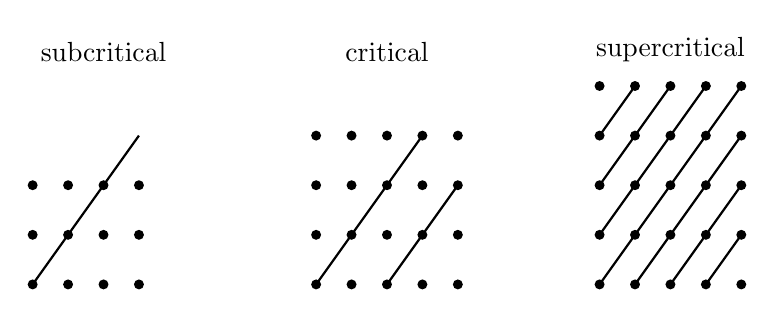
\begin{tikzpicture}[>=latex,thick,scale=0.9]
  % Subcritical
  \node[anchor=south] at (-4,3) {subcritical};
  \foreach \x in {-5,-4.5,-4,-3.5}
    \foreach \y in {0,0.7,1.4}
      \fill (\x,\y) circle (2pt);

  \foreach \x/\y in {-5/0, -4.5/0.7, -4/1.4}
    \draw (\x,\y) -- ++(0.5,0.7);

  % Critical
  \node[anchor=south] at (0,3) {critical};
  \foreach \x in {-1, -0.5, 0, 0.5, 1}
    \foreach \y in {0,0.7,1.4,2.1}
      \fill (\x,\y) circle (2pt);

  \draw (-1,0) -- (-0.5,0.7) -- (0,1.4) -- (0.5,2.1);
  \draw (0,0) -- (0.5,0.7) -- (1,1.4);

  % Supercritical
  \node[anchor=south] at (4,3) {supercritical};
  \foreach \x in {3,3.5,4,4.5,5}
    \foreach \y in {0,0.7,1.4,2.1,2.8}
      \fill (\x,\y) circle (2pt);

  \foreach \x in {3,3.5,4,4.5}
    \foreach \y in {0,0.7,1.4,2.1}
      \draw (\x,\y) -- ++(0.5,0.7);
\end{tikzpicture}

